\documentclass[letterpaper,11pt,dvipsnames]{article}	
\usepackage[mathscr]{eucal}
\usepackage[spanish]{babel}
%\usepackage[latin1]{inputenc} 
\usepackage[utf8]{inputenc} 
\usepackage{amsthm,amsmath,amssymb,amsthm,amscd,amsfonts,amsbsy}
\usepackage{mathrsfs}
\usepackage{color}
\usepackage{xcolor}
\usepackage{textcomp}
\usepackage{fancyhdr,latexsym}
\usepackage{epsfig}
\usepackage{graphicx}
\usepackage{subcaption}
\usepackage{thumbpdf}
\usepackage{float}
\usepackage{rotating}
\usepackage{setspace}
\usepackage{multicol}
\usepackage{hyperref}
\usepackage{multido}
\usepackage{multirow}
\usepackage{tabularx,booktabs,caption}
\usepackage{pgfplots}
\usepackage{curves}
\usepackage[pass]{geometry}
\usepackage[most]{tcolorbox} % Para generar textos con caja de color
\usepackage{calrsfs} %fuente caligrafica estilizada
\usepackage{listings}
\usepackage{xcolor}

\definecolor{gray}{rgb}{0.5,0.5,0.5}

\lstnewenvironment{pythoncode}[1][]{
    \lstset{
        language=Python,
        basicstyle=\ttfamily\small,
        columns=fullflexible,
        keywordstyle=\color{blue}\bfseries,
        commentstyle=\color{gray},
        stringstyle=\color{green!50!black},
        showstringspaces=false,
        numbers=left,
        numberstyle=\tiny,
        numbersep=5pt,
        breaklines=true,
        frame=single,
        frameround=tttt,
        framesep=5pt,
        backgroundcolor=\color{gray!5},
        captionpos=b,
        #1
    }
}{}
\pagestyle{plain}

\newtheorem{theorem}{Teorema}
\newtheorem{exercise}{Ejercicio}
\newtheorem{example}{Ejemplo}
\newtheorem{definition}{Definición}
%se pueden mofificar/agregar mas comandos segun los ambientes necesarios

\addtolength{\voffset}{-1.0in} 
\addtolength{\hoffset}{-1.0in}
\addtolength{\textwidth}{2.0in} 
\addtolength{\textheight}{1.751in}

\title{Círculos en círculos }
\author{Maximiliano Barajas Sánchez}
\begin{document}
\maketitle

%los logotipos oficiales de la institucion se pueden descargar desde
% https://www.comunicacionsocial.uam.mx/identidaduam/html/descargas.html
\begin{picture}(1,1)(0,0)
\put(0,90){
\includegraphics[scale=0.485,keepaspectratio=true]{variacion5Cua.png}}
\end{picture}


\section{Introducción}
A lo largo de esta práctica se analizarán dos tipos de trayectorias de gran relevancia geométrica, se trata de las hipocicloides y epicicloides. Comenzaremos introduciendo las definiciones de ambos objetos para mas adelante compartir observaciones sobre simulaciones realizadas a través de software y una implementación sencilla realizada en Python.

\section{Metodología}
En cuanto a los datos a utilizar en esta practica en particular nos centramos en epicicloides e hipocicloides en su forma paramétrica con una serie de relaciones establecidas entre los parámetros de las curvas para experimentar, se utilizó una aplicación de espiró-grafo en línea como Python para como herramientas principales de esta práctica yo decidí utilizar las librerias de Numpy y Plotly, a continuación analizaremos el fundamento teórico de la práctica.
\subsection{Fundamento Teórico}
Comenzaremos definiendo las hipocicloides, este tipo de curvas consisten en la trayectoria generada por un punto de una circunferencia que rueda dentro de otra circunferencia de radio mas grande, a lo largo de este apartado nos referiremos al radio mas grande como $a$ y al pequeño como $b$, consideremos la siguiente imagen:



\begin{figure}[H]
    \centering
    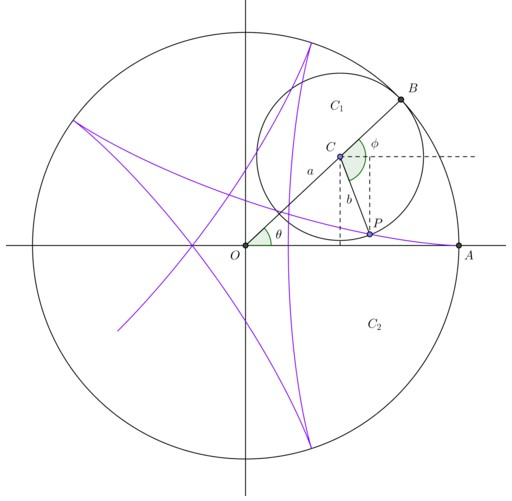
\includegraphics[scale=0.485]{hipocicloide.jpg}
    \caption{Hipocicloide auxiliar para la obtención de las ecuaciones paramétricas de las hipocicloides}
    \label{fig:hipocicloide}
\end{figure}

De la figura anterior podemos extraer en primera instancia las siguientes ecuaciones para cada coordenada mediante proyecciones sobre el eje $x$ y el eje $y$ respectivamente:
\[
x=(a-b)cos(\theta)+bcos(\phi - \theta)
\]
\[
y=(a-b)sin(\theta)-bsin(\phi-\theta)
\]

Los primeros términos, $(a-b)cos(\theta)$ y $(a-b)sin(\theta)$ vienen de proyectar la distancia del origen al punto $C$ o bien el centro de la circunferencia menor la cual esta sujeta al movimiento sobre el eje $x$ y el eje $y$ respectivamente, homologamente si proyectamos el segmento del centro del círculo de radio menor al punto $P(x,y)$ obtenemos los términos $bcos(\phi - \theta)$ y $bsin(\phi-\theta)$ para $x$ y $y$ respectivamente, se realiza la diferencia de los ángulos $\phi$ y $\theta$ dado que es el ángulo perteneciente al triángulo rectángulo formado por $b$ como su hipotenusa y los segmentos punteados como el resto de sus catetos.
Para encontrar el ángulo $\phi$ basta con darnos cuenta que el arco entre los puntos $P$ y $B$ es de misma longitud que el arco definido entre $A$ y $B$ de lo cual podemos concluir la siguiente relación:
\[
b\phi=a\theta
\]
\[
\phi=\frac{a\theta}{b}
\]
De lo anterior se sigue lo siguiente:
\[
\phi-\theta=\frac{a\theta}{b} - \theta = \theta (\frac{a}{b} - 1) = \theta \frac{a-b}{b}
\]
Finalmente obtenemos las siguientes expresiones para las coordenadas $x$ y $y$:
\[
x=(a-b)cos(\theta)+bcos(\theta \frac{a-b}{b})
\]
\[
y=(a-b)sin(\theta)-bsin(\theta \frac{a-b}{b})
\]
Tal como establecen George F. Simmons y ProofWiki
\subsection{Experimentación inicial con el espirografo}
Inicialmente probé con el espirógrafo en línea el cual es accesible a través del siguiente  \href{https://nathanfriend.io/inspiral-web/}{link} obteniendo el siguiente patrón:
\begin{figure}[h]
    \centering
    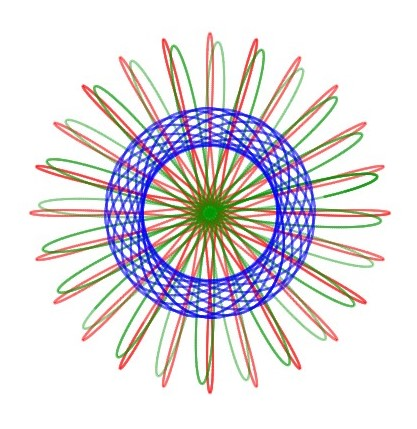
\includegraphics[scale=0.485]{espiro1 (1).jpg}
    \caption{Ejemplo de patrón realizado con el espirógrafo virtual}
    \label{fig:sample}
\end{figure}

\subsection{Implementación en Python}
Personalmente decidí modularizar el código con ayuda de una función la cual fuese la encargada de realizar el proceso de generar la gráfica de la hipocicloide y mostrarla a partir de únicamente los parámetros, decidí hacer uso de la biblioteca Plotly dado que permite generar gráficas interactivas las cuales son a mi parecer también mas atractivas que las realizadas por matplotlib, a continuación la implementación de mi función la cual solo recibe 2 parámetros obligatorios los cuales son $a$ y $b$ que son los parámetros de las ecuaciones paramétricas de las hipocicloides.
\begin{pythoncode}[caption={Implementación de la función para mostrar hipocicloides dados solamente $a$ y $b$}]
import numpy as np
import plotly.graph_objects as go
from plotly.subplots import make_subplots
from random import choice
def mostrar_curva(a: np.float64, b: np.float64, t: np.float64 = np.linspace(0, 200 * np.pi, 100000 + 1)) -> None:
    #Ecuaciones Parametricas de la hipocicloide
    x = (a - b) * np.cos(t) + b * np.cos(t * (a - b) / b) 
    y = (a - b) * np.sin(t) - b * np.sin(t * (a - b) / b)
    #Inicializamos un objeto subplots para poder construir la grafica
    fig = make_subplots(rows=1, cols=1)
    #Creamos nuestra grafica, el color lo decide al azar dentro de las opciones en la lista dentro del argumento del constructor
    hipocicloide = go.Scatter(x=x, y=y, mode='lines', line=dict(color=choice(['red', 'blue', 'green', 'yellow', 'black', 'magenta', 'cyan'])))
    #Agregamos la grafica al objeto figura como una trayectoria
    fig.add_trace(hipocicloide)
    fig.update_layout(
        #Le damos la misma escala para ambos ejes X y Y a la grafica
        xaxis=dict(scaleanchor="y", scaleratio=1),
        yaxis=dict(constrain="domain"),
        showlegend=False
    )
    #Mostramos la grafica
    fig.show()
\end{pythoncode}
Una vez ya poseemos la implementación podemos proceder con los resultados requeridos para la práctica.
\newpage
\section{Discusión}
En este apartado discutiremos los resultados obtenidos según las razones entre los parámetros $a$ y $b$ las cuales se nos pidieron en la práctica a realizar las hipocicloides asociadas a las mismas, inicialmente elegí $a = 3$ y $b=1$ y obtuve la siguiente gráfica:
\begin{figure}[H]
    \centering
    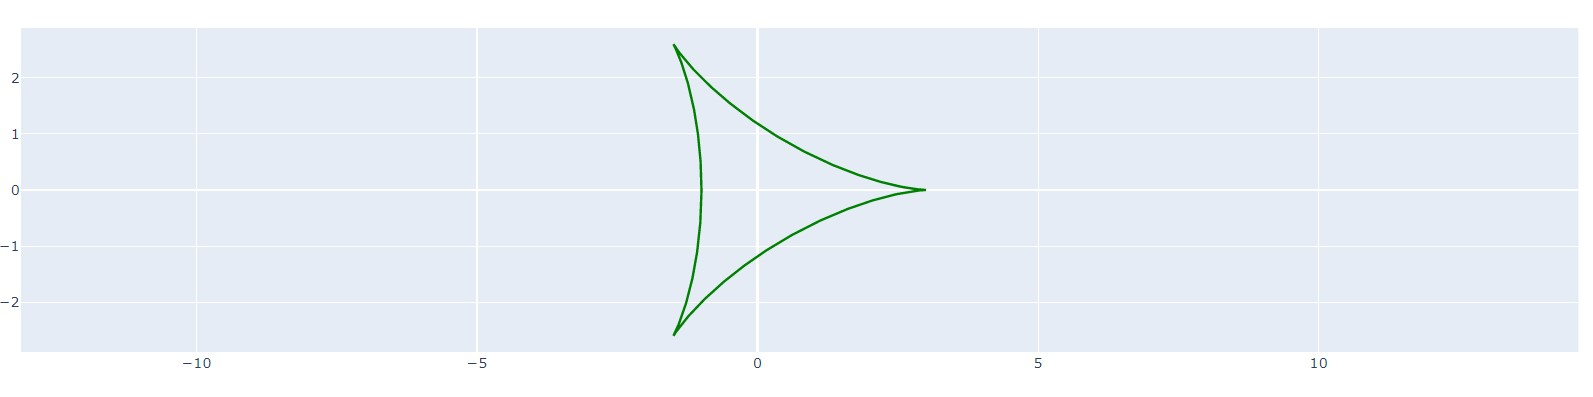
\includegraphics[scale=0.4]{grafica1.jpg}
    \caption{Hipocicloide con parámetros $a = 3$ y $b=1$ }
    \label{fig:sample}
\end{figure}
Notemos que elegí en mi caso los parámetros de esta manera para que así se cumpliera la relación de cociente establecida en la práctica, después realicé lo mismo con los parámetros $a = 4$ y $b=1$
\begin{figure}[H]
    \centering
    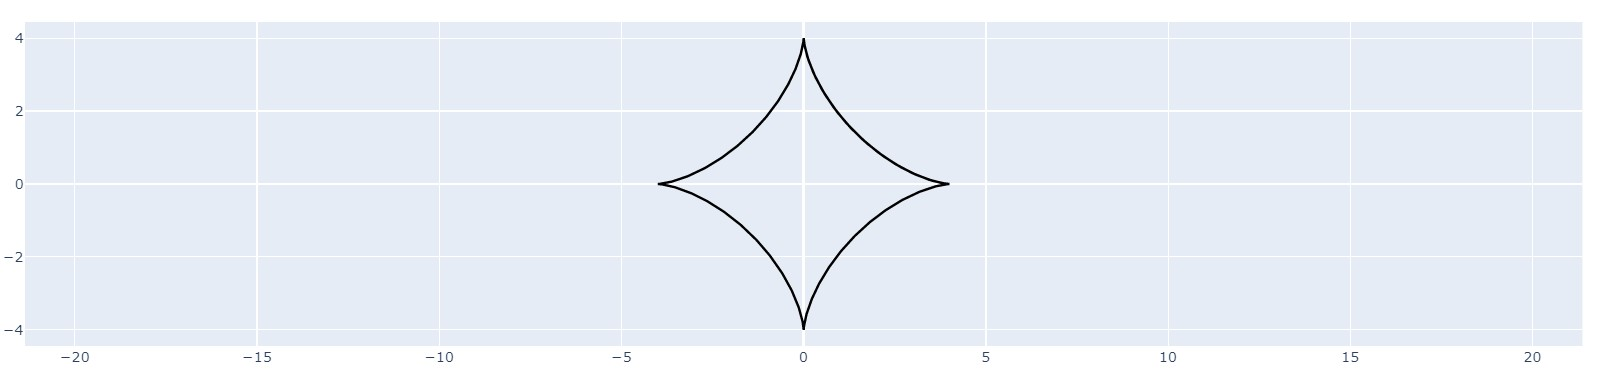
\includegraphics[scale=0.4]{grafica2.jpg}
    \caption{Hipocicloide con parámetros $a = 4$ y $b=1$ }
    \label{fig:sample}
\end{figure}
Notemos en este caso que se incrfemento el número de puntos de el patrón similar a una "estrella" formado por la trayectoria asociada a estos parámetros, sucede lo mismo si incrementamos una vez mas el parámetro $a$ en uno, que consiste en la siguiente gráfica requerida con parámetros $a = 5$ y $b=1$
\begin{figure}[H]
    \centering
    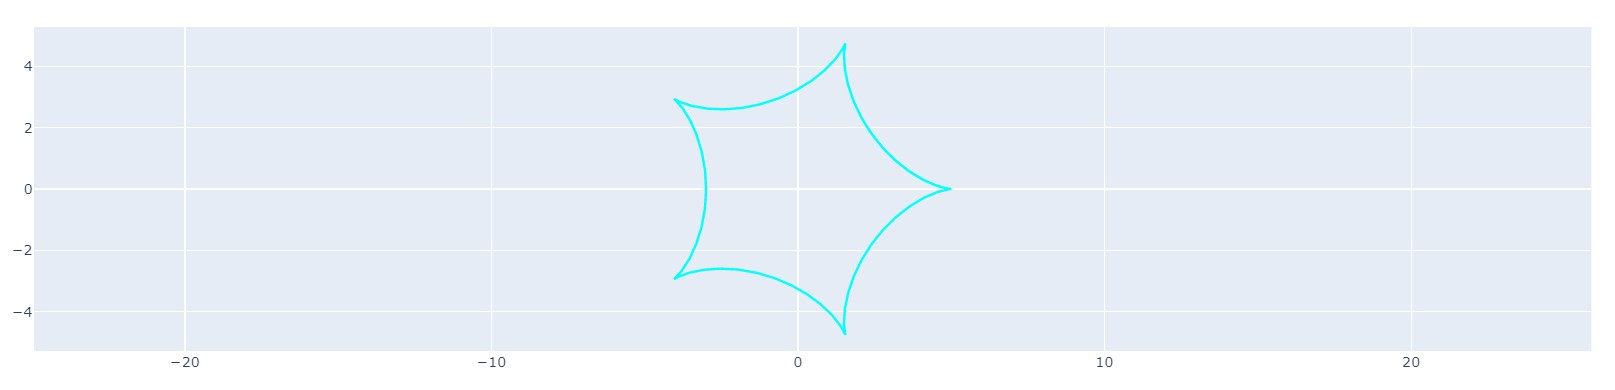
\includegraphics[scale=0.4]{grafica3.jpg}
    \caption{Hipocicloide con parámetros $a = 5$ y $b=1$ }
    \label{fig:sample}
\end{figure}
\newpage
Ahora procedemos a incrementar ambos parámetros para obtener la relación de cociente entre ellos requerida por la práctica, a continuación la hipocicloide con parámetros $a = 5$ y $b=3$ 

\begin{figure}[H]
    \centering
    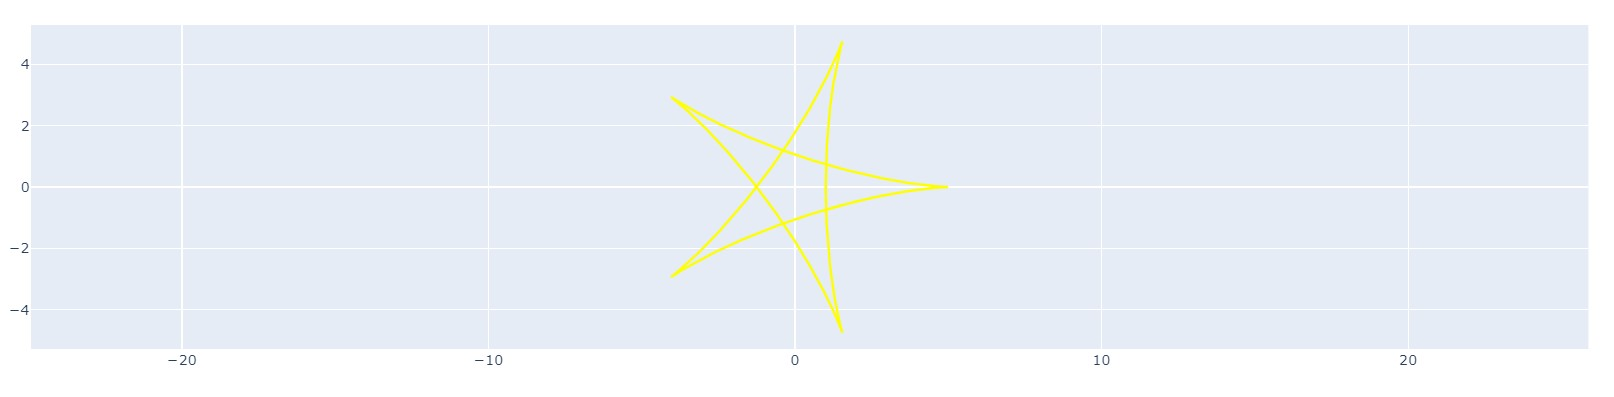
\includegraphics[scale=0.4]{grafica4.jpg}
    \caption{Hipocicloide con parámetros $a = 5$ y $b=3$ }
    \label{fig:sample}
\end{figure}
Procedemos ahora con la gráfica asociada a los parámetros $a = 7$ y $b=3$:

\begin{figure}[H]
    \centering
    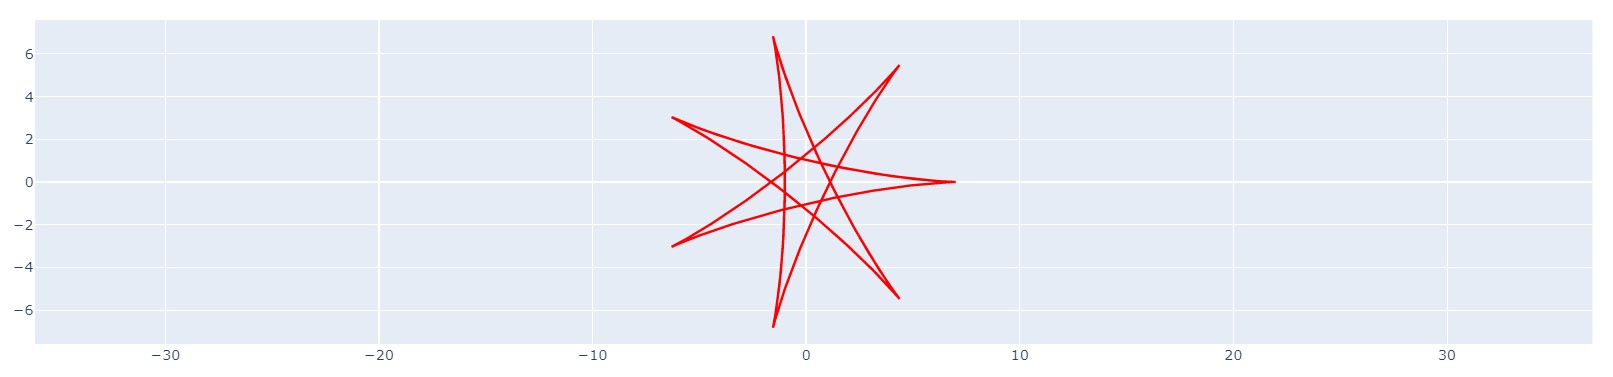
\includegraphics[scale=0.4]{grafica5.jpg}
    \caption{Hipocicloide con parámetros $a = 7$ y $b=3$ }
    \label{fig:sample}
\end{figure}
Una vez mas incrementaremos el parámetro $a$ de tal manera de que la siguiente relación requerida en la práctica se cumpla, consideremos los parámetros $a = 8$ y $b=3$, la hipocicloide asociada a estos es la siguiente:
\begin{figure}[H]
    \centering
    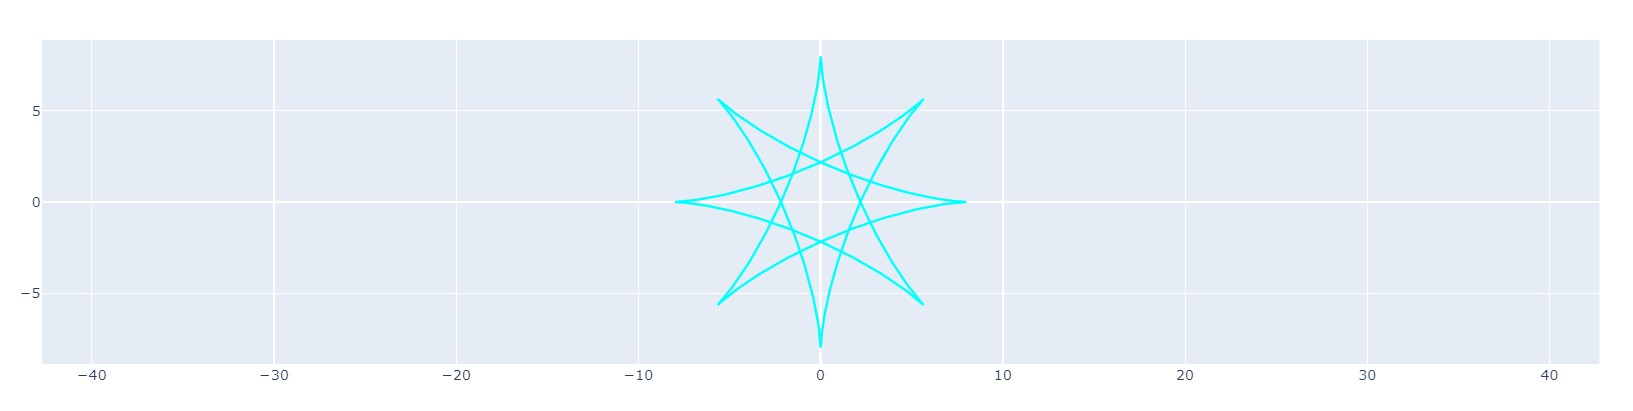
\includegraphics[scale=0.4]{grafica6.jpg}
    \caption{Hipocicloide con parámetros $a = 8$ y $b=3$ }
    \label{fig:sample}
\end{figure}
\newpage
Para los siguientes 2 casos donde se trata de una relación establecida por un irracional decidí utilizar las aproximaciones de numpy, inicialmente para la relación de cociente que es igual a $\pi$ bastó con tomar el parámetro $a=\frac{1}{\pi}$ y $b=1$ obteniendo la siguiente gráfica:
\begin{figure}[H]
    \centering
    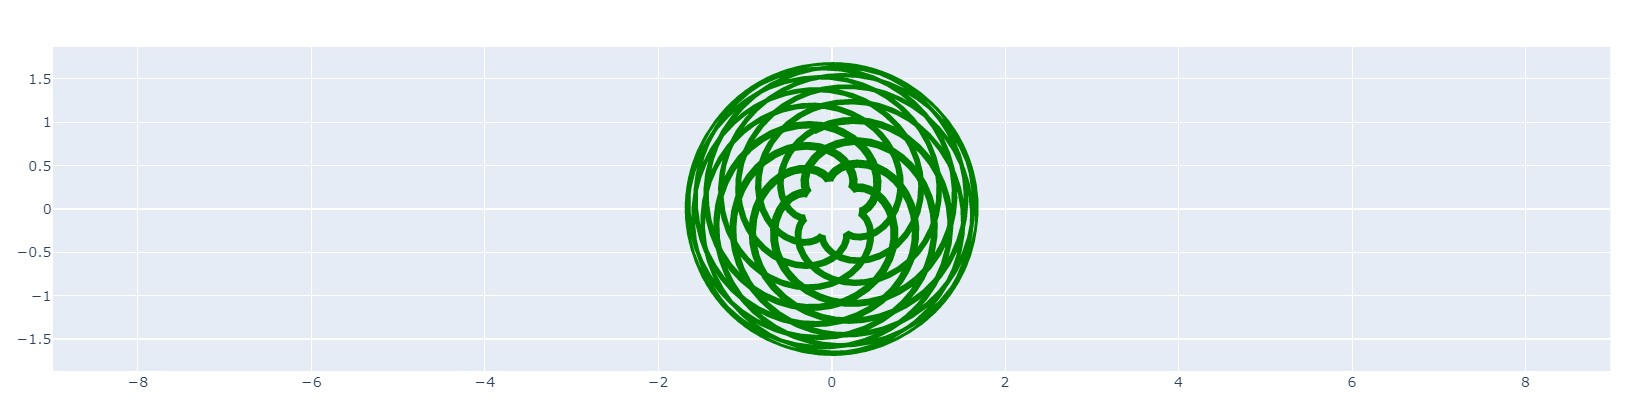
\includegraphics[scale=0.4]{grafica7.jpg}
    \caption{Hipocicloide con parámetros $a = \frac{1}{\pi}$ y $b=1$ }
    \label{fig:sample}
\end{figure}
Finalmente, de manera similar al inciso anterior decidí tomar el parámetro $a$ como $a=\frac{1}{\sqrt{2}}$ y por otra parte $b=1$ resultando en la siguiente gráfica:
\begin{figure}[H]
    \centering
    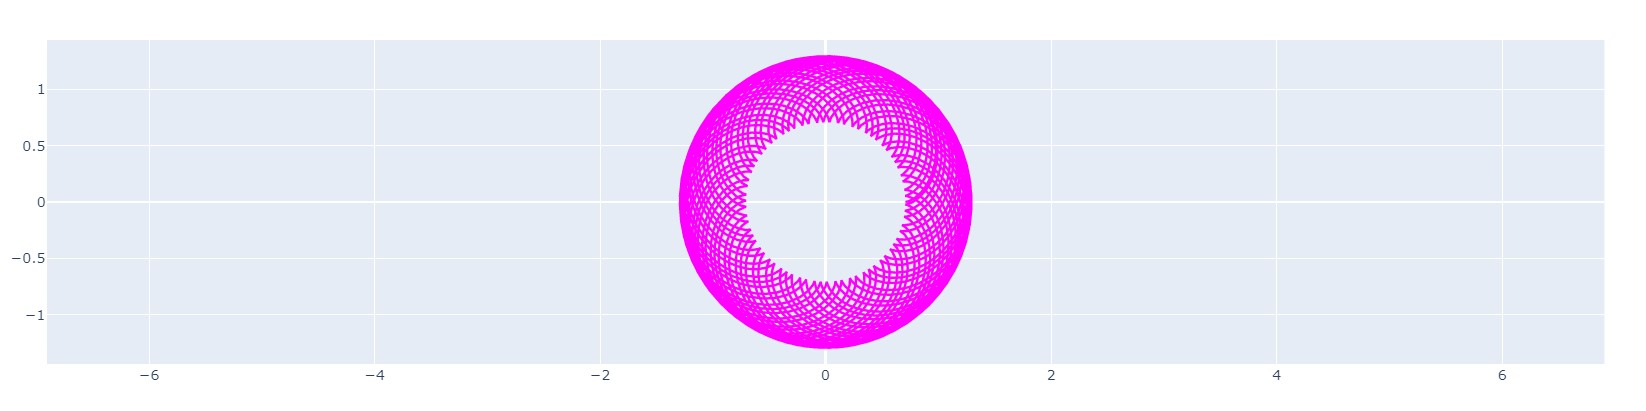
\includegraphics[scale=0.4]{grafica8.jpg}
    \caption{Hipocicloide con parámetros $a=\frac{1}{\sqrt{2}}$ y $b=1$ }
    \label{fig:sample}
\end{figure}
\section{Conclusiones} 

Finalmente podemos concluir que las hipocicloides son un objeto propio de la geometría con un estudio sobre sus características cuanto menos interesante, la peculiaridad de su aspecto me parece atractiva visualmente, sin embargo de igual manera encontré que son de gran utilidad en el diseño de sistemas rotatorios o de engranajes junto con la parametrización de algunos tipos de orbitas de cuerpos celestes en la cosmología, me pareció también muy interesante dentro de mi investigación sobre este tipo de curvas sus trayectorias homólogas que se diferencian en que la circunferencia de radio menor gira por fuera de la de radio mayor llamadas epicicloides, de igual manera Plotly me parece una excelente alternativa a matplotlib en cuanto a lo realizado en esta práctica respecta dado que originalmente realicé mis gráficas con matplotlib pero no podía realizar un zoom en específico sobre algunas de ellas o verificar si los valores erán correctos para cada trayectoria, cosa que se puede hacer solamente arrastrando el cursor con las gráficas generadas por plotly.
\newpage
\section*{Referencias Bibliográficas}
\begin{enumerate}
    \item Kühnel, W. (2015). Differential geometry (Vol. 77). American Mathematical Soc..
    \item Carver, W. B. (1956). Hypocycloids. The American Mathematical Monthly, 63(9), 58-67.
    \item George F. Simmons (1992). Calculus Gems. Chapter B.21: The Cycloid.
    \item ProofWiki. Equation of Hypocicloid \url{https://proofwiki.org/wiki/Equation_of_Hypocycloid}
    \item Weisstein, E. W. (2003). Hypocycloid. \url{https://mathworld.wolfram.com/}.
    
\end{enumerate}
\end{document}
%===========================================================================================
_______________________________FIN DEL DOCUMENTO___________________________________________
%===========================================================================================